\documentclass{article}
\usepackage{../../misc/uga-titles/uga-report-style}

\begin{document}
	\graphicspath{{../../misc/uga-titles/}}
	\report{Parking Access Control System}{Aleksandr Sergeev, login number 011}
	\graphicspath{{./}}
	
	\section*{The system}
	Below the code for parking access control system finite-state machine is listed. \\
	\ \\
	System inputs are:
	\begin{itemize}[nosep]
		\item clk: synchronization clock.
		\item reset: asynchronous reset (active high).
		\item require\_in: car driver presses the button, asking for enter.
		\item avail: there are available parking slots.
		\item timeout\_1, timeout\_2: timeout to enter, and exit parking lot.
		\item sensor\_in, sensor\_out: sensor that detects car entering and exiting the lot.
		\item insert\_ticket: car driver inserts a ticket, asking for exit.
		\item ticketOK: the inserted ticket is valid (the fee has been paid).
	\end{itemize}
	\ \\
	System outputs are:
	\begin{itemize}[nosep]
		\item gate\_in\_open, gate\_out\_open: opens gate for entering or exiting the lot.
		\item car\_in, car\_out: new car enters or exits.
		\item ticket\_inserted: ticket has been inserted.
	\end{itemize}
	\ \\
	In the code below the system is implemented as a Mealy machine.\\
	The set of states of the machine $Q = \{idle, verif\_ticket, open\_out, close\_out, open\_in, close\_in\}$. \\
	The initial state of the machine $q_0 = idle$. \\
	Machine inputs set is $I = \{0, 1\}^N$, where $N$ is the number of system inputs except "clck" and "reset", $N$ = 8. \\
	Machine outputs set is $I = \{0, 1\}^M$, where $M$ is the number of system outputs, $M$ = 5. \\
	\ \\
	The architecture of the system contains three processes:
	\begin{itemize}[nosep]
		\item Next state assignment process - used to decide, which state is next for the machine. Depends on current state and all the inputs (as a transition function $f: Q \times I \rightarrow Q$).
		\item Output assignment process - used to assign values to machine outputs. Depends on current state and all the inputs (as an output function $f: Q \times I \rightarrow O$).
		\item State switching process - used to switch machine to the next state on clock tick.
	\end{itemize}

	\lstinputlisting[language=VHDL, breaklines=true, numbers=left]{PACS.vhd}
	
	\section*{The test bench}
	Below the code for parking access control system finite-state machine test bench is listed. \\
	The test bench doesn't have neither inputs nor outputs. \\
	\ \\
	NB! Some of the test bench signal names don't match the names of the parking access system inputs and outputs. For instance:
	\begin{itemize}[nosep]
		\item require\_in \textrightarrow{} rin.
		\item timeout\_1 \textrightarrow{} t1.
		\item timeout\_2 \textrightarrow{} t2.
		\item sensor\_in \textrightarrow{} sin.
		\item sensor\_out \textrightarrow{} sout.
		\item insert\_ticket \textrightarrow{} inti.
		\item ticketOK \textrightarrow{} tiOK.
		\item gate\_in\_open \textrightarrow{} gio.
		\item gate\_out\_open \textrightarrow{} goo.
		\item car\_in \textrightarrow{} ci.
		\item car\_out \textrightarrow{} co.
		\item ticket\_inserted \textrightarrow{} ti.
	\end{itemize}
	This was done in order to reduce line length (and I regret this decision now). \\
	\ \\
	The architecture of the test bench contains the following parts:
	\begin{itemize}[nosep]
		\item Synchronization clock process. Full clock period is 50MHz, that means that a tick happens once a $\frac{1}{50 \cdot 10^6}$ of a second, or once per 20 nanoseconds. Half clock cycle is thus 10 ns.
		\item Parking access system port mapping - signals of the test bench are associated with inputs and outputs of the parking access system instance.
		\item Initial setup - the global parameters that won't be tested are set up here, these are: "reset" (is always '0'), "avail" (is always '1') and "ticketOK" (is always '1').
		\item "Car leaves" test - simulation of a car leaving parking lot process. It starts at 0 ns and ends at 70 ns. And more precisely:
		\begin{itemize}[nosep]
			\item "require\_in" is set from 0 to 25 ns.
			\item "timeout\_1" is set after 70 ns.
			\item "sensor\_in" is set from 30 to 50 ns.
		\end{itemize}
		\item "Car arrives" test - simulation of a car entering parking lot process. It starts at 80 ns and ends at 150 ns. And more precisely:
		\begin{itemize}[nosep]
			\item "inset\_ticket" is set from 80 to 100 ns.
			\item "timeout\_2" isn't set from 80 ns to 150 ns.
			\item "sensor\_out" is set from 110 to 130 ns.
		\end{itemize}
	\end{itemize}
	
	\lstinputlisting[language=VHDL, breaklines=true, numbers=left]{bench_PACS.vhd}
	
	\section*{Runtime screenshot}
	The result of the test simulation is expected to be: \\
	\ \\
	Car leaves test:
	\begin{itemize}[nosep]
		\item "gate\_in\_open" to be set from 10 to 50 ns.
		\item "car\_in" to be set from 30 to 50 ns.
		\item state "idle" to be set from 0 to 10 ns.
		\item state "open\_in" to be set from 10 to 30 ns.
		\item state "close\_in" to be set from 30 to 50 ns.
		\item state "idle" to be set from 50 to 70 ns.
	\end{itemize}
	\ \\
	Car arrives test:
	\begin{itemize}[nosep]
		\item "ticket\_inserted" to be set from 80 to 90 ns.
		\item "gate\_out\_open" to be set from 110 to 130 ns.
		\item "car\_out" to be set from 110 to 130 ns.
		\item state "idle" to be set from 80 to 90 ns.
		\item state "open\_out" to be set from 110 to 130 ns.
		\item state "close\_out" to be set from 130 to 150 ns.
		\item state "idle" to be set from 150 ns.
	\end{itemize}
	\ \\
	The results summary: \\
	While writing this report, I realized that I didn't describe the meaning of "close\_in" and "close\_out" correctly: the car is supposed to enter and exit the parking lot during these states, so I had to set "car\_in", "car\_out", "gate\_in\_open" and "gate\_out\_open" upon transition to idle state only. \\
	I also had to set "sensor\_out" on line 34 of parking access control system test bench later, from 130 to 150 ns.\\
	Moreover, on the line 51 of parking access control system description I had to set "gate\_in\_open" unconditionally. \\
	\ \\
	Because of these inaccuracies, the actual test results differ from the expected:
	\begin{enumerate}[nosep]
		\item "car\_in" gets unset too early, on 30 ns, directly after being set.
		\item "gate\_in\_open" gets unset too early, on 30 ns.
		\item "car\_out" gets unset too early, on 30 ns, directly after being set.
		\item "sensor\_out" gets set and unset too early, from 110 to 130 ns.
		\item "car\_out" gets set and unset too early, from 110 to 130 ns.
		\item "gate\_out\_open" gets set too late, on 130 ns.
		\item state "open\_out" lasts for too long - 40 ns, instead of 20.
	\end{enumerate}
	\ \\
	The result of this misunderstanding is predictable wrong, but I can't fix it because I have already handed in the picture of automaton and also I can't rerun the test outside the lab room. \\
	On the other hand, the bug of the given system was found and is clearly described above. \\
	That's all I can do now.

	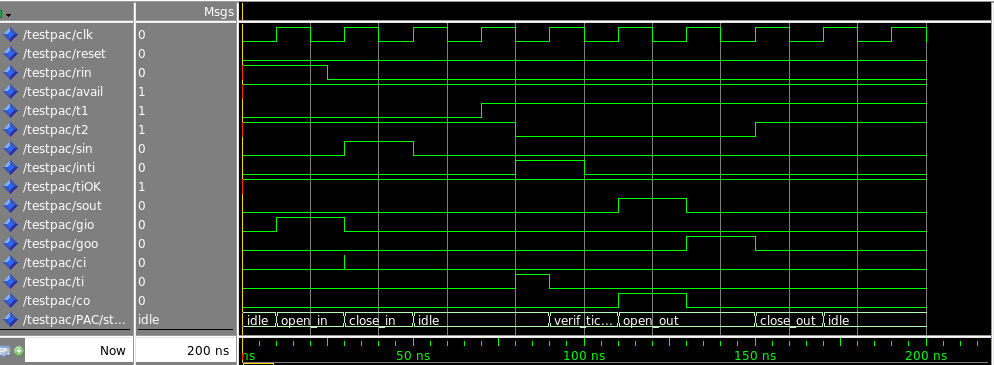
\includegraphics[width=\textwidth]{test.png}
\end{document}
